%ekg_7_Realisierung/Konzeptfindung

\subsection{Konzeptfindung}

Dieses Unterkapitel führt die Anforderungen und die gewählten Lösungen auf, ohne diese im Detail zu erklären. Die genaue Erläuterung der verfolgten und getesteten Umsetzungen sind Inhalt der folgenden Kapitel der Realisierung. 

\subsubsection{Konzeptionierung}

Zur Erstellung eines Konzeptes für das EKG-Gerät wurden zunächst alle Anforderungen die sich aus dem Signal und den Produktvorstellungen ergaben, gesammelt. Hierzu zählen auch Funktionen die über die bloße Aufzeichnung eines EKGs hinausgehen.

\begin{enumerate}
\item Bandbreite der Filterschaltung: \SI{0.5}{\hertz} - \SI{160}{\hertz}
\item Abtastfrequenz: \SI{250}{\hertz} - \SI{1000}{\hertz}
\item Benötigte Verstärkung für das EKG-Signals: \SI{66}{\decibel} (= Faktor 2000)
\item Für ein Ein-Kanal-EKG muss eine Differenzbildung der Signale zwischen den beiden Ableitungspunkten durchgeführt werden
\item Die negativen Signalanteile des EKGs müssen mit einer unipolaren Versorgungsspannung übertragen werden
\item Durch Magnetfelder von umgebenden Versorgungsleitungen induzierte Störsignale (sogenanntes Netzbrummen) müssen unterdrückt werden
\item Die verwendeten aktiven elektronischen Bauteile müssen mit einer unipolaren Versorgungsspannung betrieben werden können und sollten diesen Spannungsbereich fast vollständig ausnutzen
\item Zur Anzeige des Signals soll wahlweise ein integriertes Display oder das eigene Smartphone verwendet werden
\item Die Bedienung erfolgt via Touchscreen mit einem intuitiven User-Interface
\item Als Aufnahmemodi werden ein Kurzzeit-EKG (\SI{2}{\min}) und ein Langzeit-EKG (24 Stunden) angeboten
\item Die Betriebslaufzeit muss mindestens 30 Stunden betragen
\item Die Energieversorgung erfolgt über einen Lithium-Ionen-Akku
\item Die aufgenommenen Daten werden auf einem externen Speichermedium gesichert
\item Bei einem niedrigen Akkustatus soll das Gerät den Nutzer durch einen akustischen Warnton darauf hinweisen
\end{enumerate}

Die Bandbreite wurde nach der Analyse eines künstlichen Testsignals (siehe Abbildung \ref{fig_Matlab EKG-Signal}) mithilfe von Matlab gewählt. Das EKG-Signal wurde aus Kosinus- und linearen Funktionen erstellt und danach durch eine Fast-Fourier-Transformation (FFT) das Frequenzspektrum (siehe Abbildung \ref{fig_Matlab Frequenzspektrum}) ermittelt. Die betragsmäßig größten Frequenzanteile reichen von \SI{0}{\hertz} bis etwa \SI{40}{\hertz}. Da jedoch gerade die hochfrequenten Anteile des Signals für die Ausformung der charakteristischen QRS-Zacken verantwortlich sind, wurde die Grenzfrequenz der Tiefpassfilterung auf \SI{160}{\hertz} gesetzt. Der Gleichanteil des Signals wird mit einem Hochpass abgetrennt und das Wechselsignal auf ein DC-Potenzial von etwa \SI{1,5}{\volt} überlagert. Dadurch dass die Filterschaltung auf ein Gleichspannungspotenzial von $\frac{V_{cc}}{2}$ angehoben wird, ist es möglich auch negative Signalanteile mit der einseitigen positiven Versorgungsspannung zu übertragen.

\begin{figure} [!h]
	%\centering
	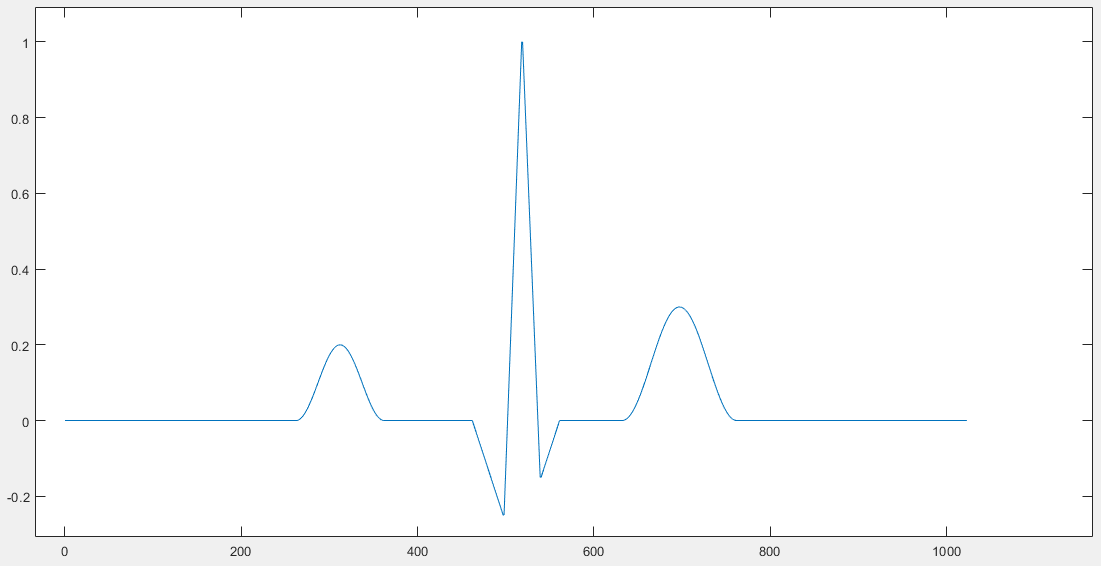
\includegraphics[width=\textwidth] {EKG_Signal.png}
	\caption{mit Matlab erstelltes künstliches EKG-Signal}
	\label{fig_Matlab EKG-Signal} 
\end{figure}

\begin{figure} [!h]
	%\centering
	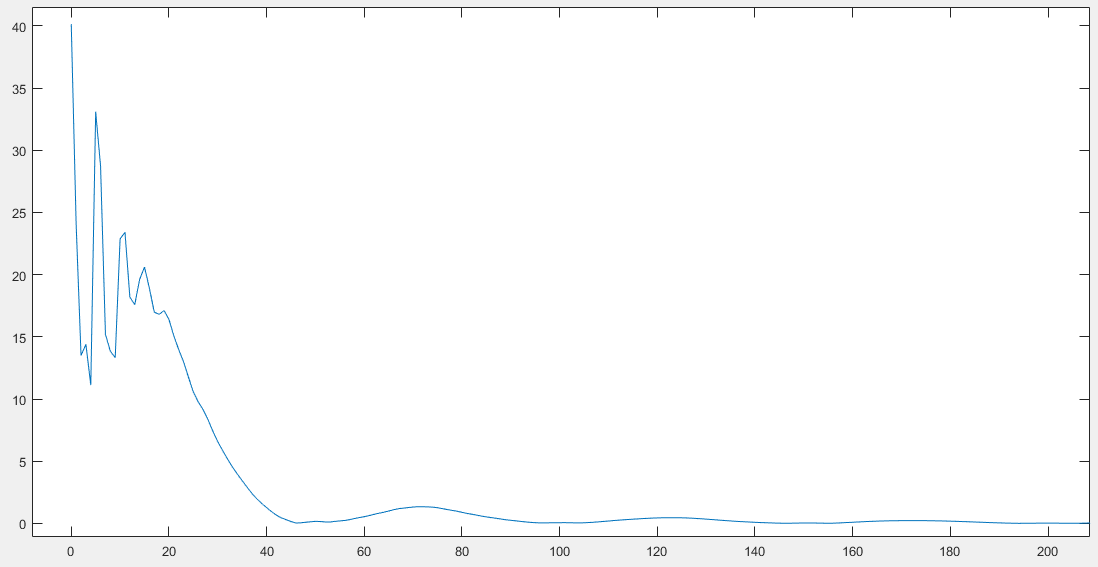
\includegraphics[width=\textwidth] {EKG_diskretes_Frequenzspektrum_Ausschnitt.png}
	\caption{Frequenzspektrum des künstlichen EKG-Signals}
	\label{fig_Matlab Frequenzspektrum} 
\end{figure}

Da das Störsignal durch Magnetfelder mit der gleichen Frequenz der Versorgungsleitungen schwingt, wird das EKG-Signal durch Kerbfilter mit einer Sperrfrequenz von \SI{50}{\hertz} gefiltert. Zur Differenzbildung der beiden Eingangskanäle wird ein Instrumentenverstärker eingesetzt. Gleichzeitig dient er zur Vorverstärkung des Signals um die Störanfälligkeit gegen elektromagnetische Felder auf dem Weg durch die Schaltung zu reduzieren. Am Ende erfolgt eine Nachverstärkung um den Arbeitsbereich und somit auch die Auflösung des ADC bestmöglich auszunutzen. Abbildung \ref{fig_Blockschaltbild Filter} zeigt die einzelnen Stufen der Filterung schematisch.

\begin{figure} [!h]
	%\centering
	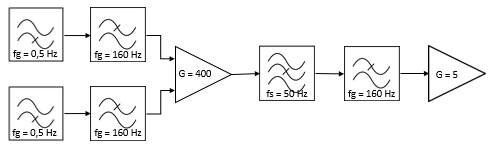
\includegraphics[width=\textwidth] {Filter Blockschaltbild.png}
	\caption{Blockschaltbild der Filterschaltung}
	\label{fig_Blockschaltbild Filter} 
\end{figure}

%Konzept Versorgung:
Wie aus Abbildung \ref{fig_Blockschaltbild} zu erkennen ist, werden zwei Versorgungsspannungen (\SI{3}{\volt}  und \SI{5}{\volt}) für die Module benötigt. Sie werden aus dem Spannungsbereich eines Lithium-Ionen-Akkus mithilfe eines LDO für \SI{3}{\volt} und eines Aufwärtswandlers für \SI{5}{\volt} erzeugt. Die Konzeptfindung der Spannungsversorgung wird im Folgendem erläutert.

Für die Wahl des Akkumulators ist die geforderte Laufzeit von mindestens 30 Stunden sowie die Stromaufnahme der Unterbaugruppen ausschlaggebend. Letztere setzt sich wie folgt zusammen:\\

\begin{tabular}[h]{l|c|r}
Komponente & Nennspannung & Stromverbrauch während Langzeitaufnahme\\
\hline
Display & 5 V & 10 mA \\
Bluetooth & 5 V & 8 mA \\
Cardreader & 5 V & 15 mA \\
MCU & 3 V & 4 mA \\
Signalfilterung & 3 V & 3 mA \\
\end{tabular}\\

Resultierend daraus eribt sich die gesammte Leistungsaufnahme zu: 
\[ P_{sum} = 5\,\mbox{V} \cdot (10\,m \mbox{A} + 8\,m\mbox{A} + 15\,m\mbox{A}) + 3\,\mbox{V} \cdot (4\, m\mbox{A} + 3 \,m\mbox{A}) = 186\, m\mbox{W} \]

Die Effizienz der noch unbekannten Spannungswandler wird vorläufig mit 80\% angenommen:
$$ P_{Akku} = 186\,m\mbox{W} \cdot \frac{1}{0.8} = 232.5\,m\mbox{W} $$

Multipliziert man den Leistungsbedarf mit der gewünschten Laufzeit, so ergibt sich eine nötige Energiemenge von:
$$ E_{Akku} = 232.5\,m\mbox{W} \cdot 30\,h = 6975\,m\mbox{W}h $$

Die Nennspannung dieser Zellen beträgt \SI{3,7}{\volt}. Dadurch ergibt sich eine nötige Ladungsmenge von: 
$$ Q_{Akku} = \frac{6975\,m \mbox{W} h}{3.7\,\mbox{V}} = 2051\,m\mbox{A}h $$

Diese Ladungsmenge wird großflächig über die Zellgröße 18560 angeboten, welche Weltweit in Massenfertigung produziert wird und somit keine Finanziellen oder Logistische Probleme darstellt.

Lithium-Ionen Zellen nehmen während ihrer Entladung Spannungen zwischen 4.2 V und 3.2 V abhängig vom Ladezustand an. Da sich aus diesem weiten Bereich die Komponenten des EKG-Gerätes nicht zuverlässig versorgen lassen, müssen stabile Zwischenspannungen erzeugt werden. Die erzeugten Spannungen müssen in der Lage sein den maximalen Strom für ihre Baugruppen zu liefern, welcher sich wie folgt zusammensetzt:\\

\begin{tabular}[h]{l|c|r}
Komponente & Nennspannung & Stromverbrauch maximal\\
\hline
Display & 5 V & 100 mA \\
Bluetooth & 5 V & 40 mA \\
Cardreader & 5 V & 100 mA \\
MCU & 3 V & 7 mA \\
Signalfilterung & 3  V & 3 mA \\
\end{tabular}\\

Dies ergibt eine Stromaufnahme von: $ I_{3\,V} = 10\,m\mbox{A}$ und $I_{5\,V} = 240\,m\mbox{A} $ \\

Für die Erzeugung von 5 V wird ein Aufwärtswandler verwendet. Hierbei handelt es sich um eine integrierte Schaltungen, welche durch zerhacken einer Gleichspannung eine DCDC Wandlung auf höhere Spannungen ermöglicht. Diese ICs sind platzsparend, da sie bereits im SOT23 Package erhältlich sind, und können problemlos Ströme im einstelligen Amperebereich bereitstellen. \\

Die Generierung von 3V durch einen Abwärtswandler ist möglich, allerdings weist diese Schaltungsart bauartbedingt eine Restwelligkeit auf. Da die komplette Analogschaltung zur Aufnahme es EKG Signals mit 3V versorgt wird, soll hier jede Form von Schwankung vermieden werden.
Deshalb fällt die Wahl für die Generierung von 3V auf einen LDO (Low-Dropout-Regler), welcher einen Spannungsabfall über einen internen MOS-FET verursacht und somit die Eingangsspannung auf eine festgelegte Ausgangsspannung herunter regelt. Da in einem LDO keine schaltenden Vorgänge Stattfinden, ist die Restwelligkeit sehr gering.\\

Die Anzeige und Steuerung erfolgt über ein 3,2 Zoll TFT Touch Display. Es verfügt über eine serielle Schnittstelle und kommuniziert via UART mit dem Input/Ouput-Modul des Prozessors. Zur zusätzlichen Bedienung wurde ein Taster eingeplant, der zum Ein- und Ausschalten des Energiesparmodus verwendet wird. Der Buzzer dient für akustische Warnsignale bei Fehlfunktion oder einem niedrigen Ladezustand des Akkus.\\

Die zweite UART-Schnittstelle (Universal Asynchronous Receiver Transmitter) der CPU wird verwendet um Daten an das Bluetooth-Modul zu senden. Dieses kommuniziert dann via Bluetooth mit dem Smartphone des Benutzers, um die EKG-Daten in der App anzuzeigen.\\

Die Datenspeicherung erfolgt auf einer externen SD-Karte. Das Kartenmodul das zum Schreiben und Lesen der Daten verwendet wird, kommuniziert via SPI (Serial Peripheral Interface) mit dem Input/Output-Modul der CPU.\\

Zur Programmierung und Fehleranalyse der Prozessoreinheit auf der Platine, wird die JTAG-Schnittstelle (Joint Test Action Group) verwendet.\\

%Konzept Display:
Das Display und dessen User Interface (UI) wurde mithilfe von vergleichbaren Geräten anhand einer Marktrecherche und anhand der Funktionalitäten des Lastenheftes konzeptioniert. Das UI ist mit der Nextion-Editor Software entwickelt und programmiert worden. Diese Software verfügt über eine übersichtliche Benutzerumgebung und einer eigenen Programmiersprache. Die Befehle und Anweisungen der Nextion Programmiersprache sind auf der offiziellen Homepage vorzufinden. Auf der Homepage sind auch allgemeine Regeln und Praktiken im Umgang mit dem Display aufgezeigt.
\\

%Konzept MCU:
Das Projekt EKG7 basiert auf dem Microcontroller MSP430F5529. Laut der Projektvorgaben muss der Prozessor zur MSP430-Prozessorfamilie der Firma Texas Instruments gehören. Nach der Analyse verschiedener µC fiel die Wahl auf die MSP430F5529. Dieser Mikrocontroller hat alle notwendigen Spezifikationen, um die Anforderungen im Lasten- und Pflichtenheft zu erfüllen.\\
Das Hauptziel der Baugruppe ist eine kontinuierliche und unterbrechungsfreie Bearbeitung und Übertragung des analogen Eingangssignal an verschiedene Module mit einem möglichst niedrigen Stromverbrauch.\\
F5529 MCU verfügt über fünf verschiedene Stromsparmodi. In diesen Modi liegt die Stromaufnahme im µA-Bereich. Der aktive Zustand des Prozessors verbraucht bei maximaler Belastung im „Worst Case“ 3,7 mA.\\
Der nächste wichtige Aspekt ist eine ausreichende Taktfrequenz. Die maximale Frequenz der F5529 beträgt 25 MHz. In diesem Projekt sind die Clocks auf eine Frequenz von 20 MHz eingestellt.\\
Die MCU verfügt über 2 UART- und 4 SPI-Schnittstellen. Beide UART Schnittstellen sind für Bluetooth-Verbindung und Kommunikation mit dem Display ausgelegt. Eine SPI-Schnittstelle ist für die Datenübertragung an das Bluetooth Modul verwendet.
Die ADC Schnittstelle hat die Auflösung von 12-bit, was möglich macht die Werte im Bereich von 0 bis 4095 zu empfangen. Das ermöglicht sowohl eine präzise Aufnahme eines EKG-Signals als auch präzises Ablesen der Akku-Werte mit einem gewissen Offset.\\ 
Ein weiterer Faktor für diese Projektarbeit ist die Anzahl der I/O Pins. Die MCU besitzt insgesamt 63 GPIO Pins inklusive 16 interruptsfähige Pins. Dies erleichtert das Hardwaredesign und gibt mehr Freiheit bei der Codeentwicklung.\\
Die MCU besitzt 8kB RAM. Der Speicher ist genügend, um die temporären Werte intern auf der MCU zu speichern und diverse Features wie z.B. digitale Filterung zu testen.\\
Ein entscheidender Faktor bei der MCU Auswahl ist die Verfügbarkeit von DevKit mit der gleichen MCU. Nach der Codeentwicklung auf dem DevKit ist es möglich die entwickelte Software mit minimalen Codeanpassungen auf das PCB zu portieren.\\

Als Grundstruktur des Codes wird eine State Machine implementiert. Diese besteht aus verschiedenen Zuständen. Jeder Zustand kann als Modul separat programmiert und getestet werden. Dies vereinfacht die Codeentwicklung, erschafft Codeübersichtlichkeit, ermöglicht die Entwicklung verschiedenen Zustände und Bedingungen, unter welchen ein Zustand gewechselt werden kann. In einer State Machine ist es immer möglich festzustellen, in welchem Zustand das Programm sich befindet.\\

\begin{figure} [h]
	%\centering
	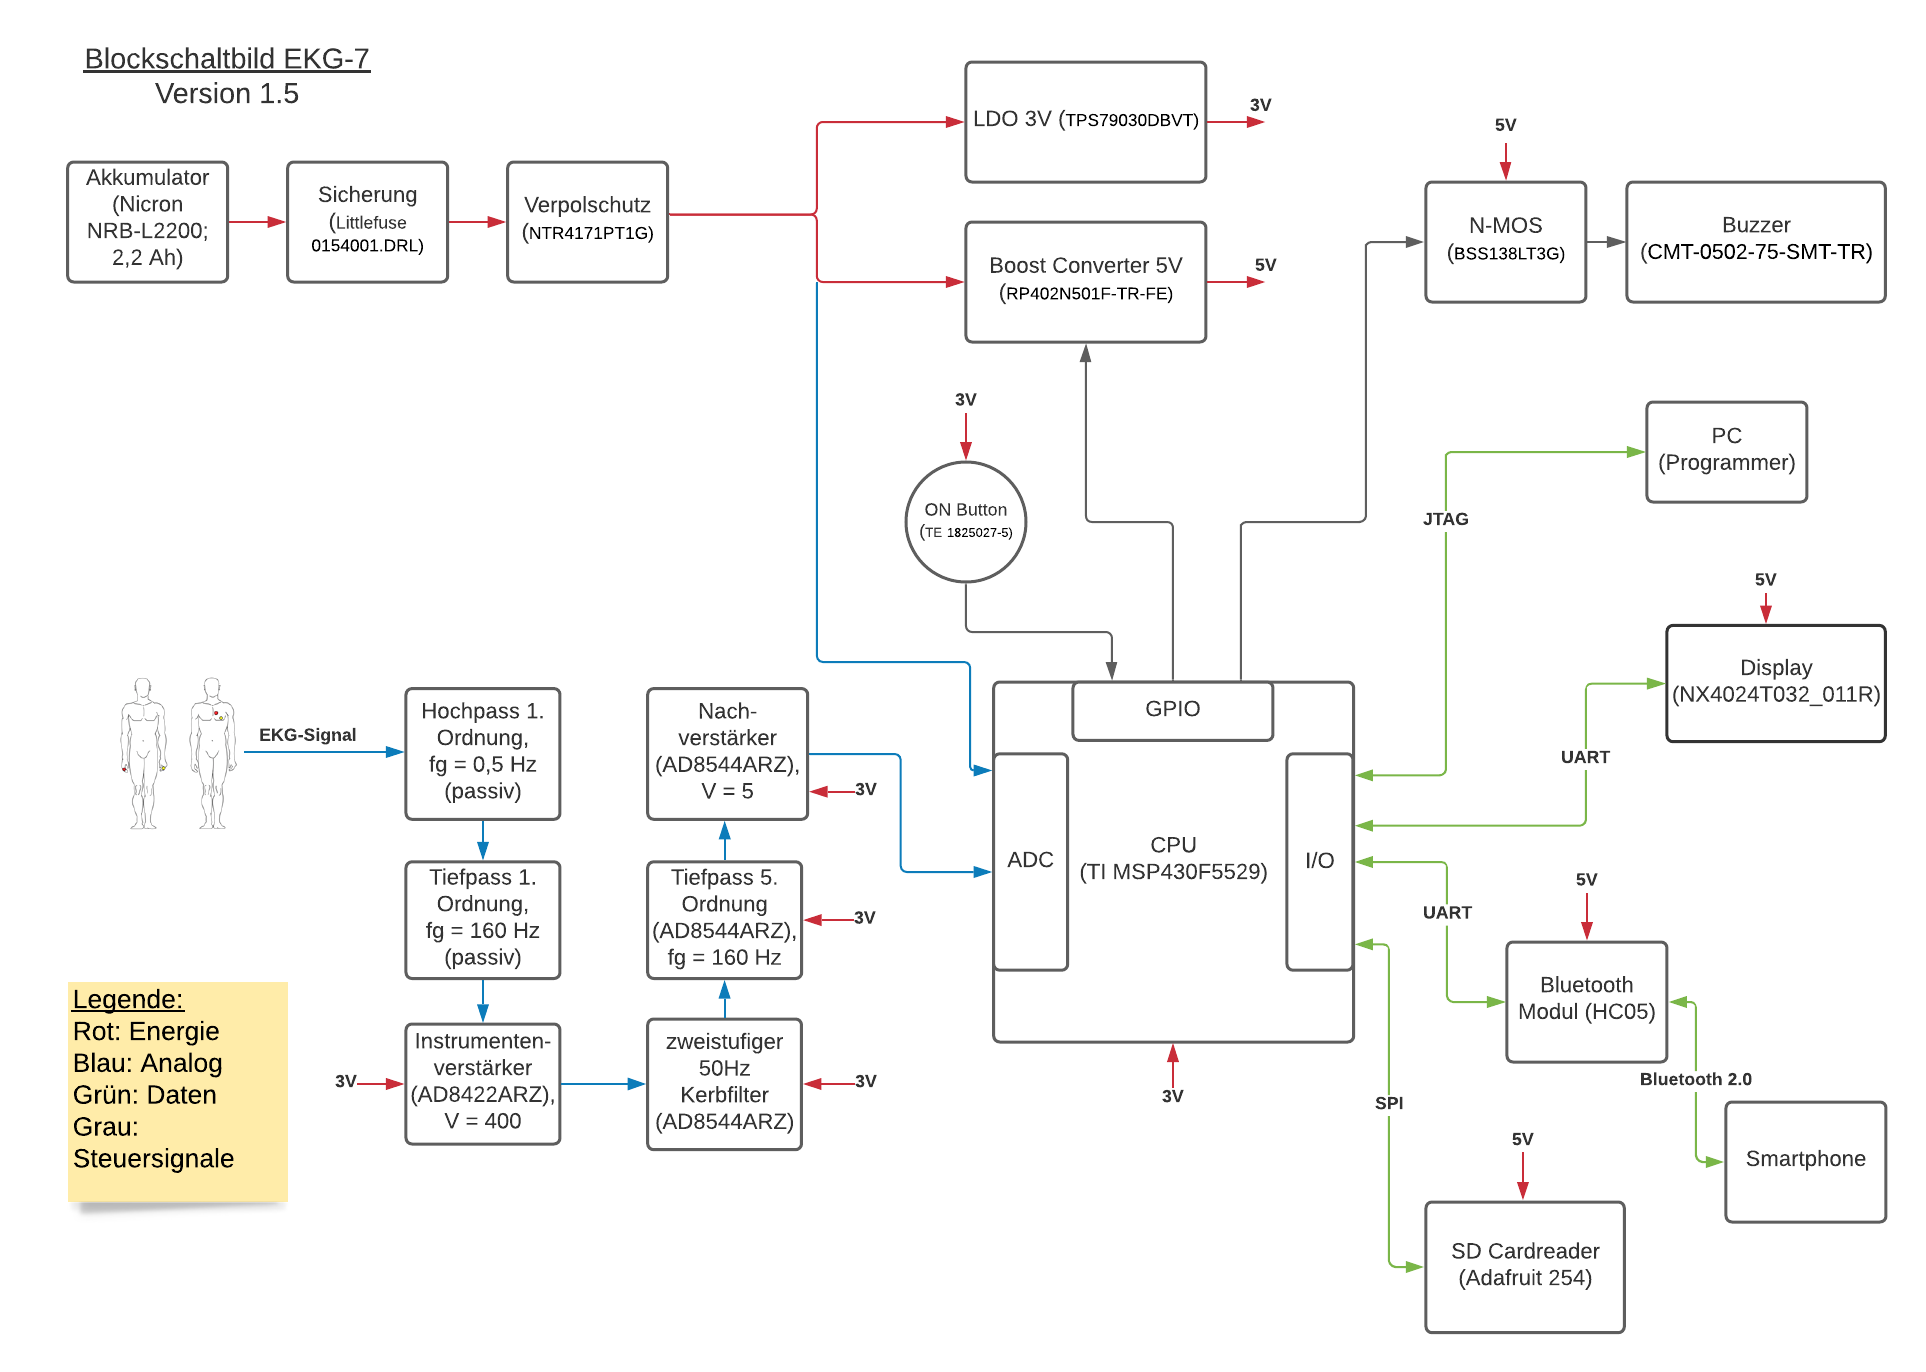
\includegraphics[width=\textwidth] {Blockschaltbild v1.5.png}
	\caption{Blockschaltbild des EKG-Geräts}
	\label{fig_Blockschaltbild} 
\end{figure}


%TODO PROJEKTGRUPPE: Konzeptionierung der jeweiligen Baugruppe; Gründe warum die jeweiligen Bauteile verwendet wurden noch hinzufügen

\subsubsection{Verwendete Software}
Für die Erstellung und Frequenzanalyse eines künstlichen EKG-Signals wurde das numerische Rechentool Matlab verwendet. Damit konnten die Grenzfrequenzen des Signals bereits ohne Labortest abgeschätzt werden. Diese Erkenntnisse wurden bei der Schaltungsentwicklung der analogen Filterschaltung mit LTSpice angewandt. Durch die Einbindung von Herstellermodellen, war die Simulation von Bauteilen möglich, ohne diese physisch zu testen. Für den Entwurf der Leiterplatine kam Altium Designer zur Anwendung. Auch hierfür bieten Hersteller Modelle für die Pinbelegung, den Footprint und 3D-Modelle an. Besonders die 3D-Modelle waren für das Gehäusedesign hilfreich um die korrekte Lage und Maße der Bauteile im Gehäuse auch optisch zu prüfen.\\
Für das Display wurde die Software Nextion-Editor verwendet. Diese Software ist speziell für das Display angefertigt und kann beim gleichnamigen Hersteller heruntergeladen werden. Der Nextion-Editor verfügt über ein weites Spektrum von Tools. Für die jeweiligen Symbole der Benutzeroberfläche wurde mit GIMP gearbeitet. Anhand der Symbole ist die UI in allen Bereichen visuell aufeinander abgestimmt.\\
Der Code ist im IDE Code Composer Studio entwickelt. CCS ist ein Produkt der Firma Texas Instruments. Das IDE ist Eclipse-basiert, besitzt eigenen Compiler, Programmierumgebung und die Möglichkeit im Debug-Modus auf einzelne Register der MCU zuzugreifen.\\
Für Version Control ist ein privates Repository auf GitHub eingestellt. Damit lässt sich die Codeentwicklung sowohl von einzelnen Modulen als auch von dem ganzen Projekt zu verfolgen.\\
%TODO PROJEKTGRUPPE: weitere Software die wir verwendet haben wie Blender, Nextion Editor, CCS, Git, Android Studio etc...

\subsubsection{Verwendete Geräte}
%TODO Geräteliste: LaunchPad, Debugger (JTAG), Arduino (Testen von SPI)...
Das LaunchPad MSP-EXP430F5529LP ist für das Testen des entwickelten Codes verwendet. Das LaunchPad verfügt über die MCU MSP430F5529. Die Schnittstellen, die dieser µC besitzt, sind auf der LaunchPad-Platine verteilt und mit Pinleisten vorgesehen. Somit lässt sich die Peripherie mithilfe von Kabeln und Jumpers anschließen und testen. Anhand dieser Tests wurde die Funktionalität diverser Schaltungen geprüft. Das LaunchPad verfügt über eine interne Debugger-Einheit, sodass die MCU sich via USB Verbindung mit einem Rechner  flashen und debuggen lässt.\\
Für das Flashen und Debuggen ist eine JTAG-Schnittstelle auf dem PCB vorgesehen. Da das PCB für die Massenfertigung entwickelt ist, ist die Debugger-Einheit wegen Kostenersparnis nicht mehr vorhanden. Die MCU wird direkt via eine JTAG-Schnittstelle durch eine externe Debugger-Einheit angesprochen.\\
Bei der Codeentwicklung kam Arduino Nano als Slave-Einheit zum Einsatz. Damit wurde die SPI Verbindung zum µC F5529 getestet. 
\subsubsection{Bauteilbeschaffung und Fertigung} 